% \documentclass[a4paper]{extreport}
\documentclass[a4paper]{scrartcl}

% Use Times NR as font
\usepackage{lmodern}
\usepackage[T1]{fontenc}

% set page margins
\usepackage[left=2cm,right=2cm,top=2.5cm,bottom=2.5cm]{geometry}

% fix for pandoc build
\providecommand{\tightlist}{\setlength{\itemsep}{0pt}\setlength{\parskip}{0pt}}

% set some variable
\newcommand{\Title}{Summary Deep Learning}
\newcommand{\Modul}{TSM\_DeLearn}
\newcommand{\Subtitle}{Master of Science in Engineering}
\newcommand{\Author}{Andrin Bürli, Nursinem Dere, Fabian Gröger}
\newcommand{\Date}{\today}

% set document properties
\title{\Title}
\date{\Date}
\author{\Author}
\subtitle{\Subtitle}

% include package to get page count
\usepackage[lastpage,user]{zref}

% include package for links
\usepackage[hidelinks]{hyperref}

% include package to setup page header and footer
\usepackage{fancyhdr}

% set page header and footer
\pagestyle{fancy}
\lhead{\Title}
\rhead{\Author}
\lfoot{\Modul}
\cfoot{\Date}
\rfoot{page \thepage\ of \zpageref{LastPage}}

% add line between page header and content
\renewcommand{\headrulewidth}{0.4pt}

% add line between page footer and content
\renewcommand{\footrulewidth}{0.4pt}

% use utf8 for special chars
\usepackage[utf8]{inputenc}

% package for better table support
\usepackage{longtable,booktabs}

% position table left and not centering
\setlength\LTleft\parindent
\setlength\LTright\fill

% disable paragraph indentation
\setlength{\parindent}{0mm}

\usepackage[table]{xcolor}

% package for code listenings
\usepackage{minted}
\usepackage{mdframed}
\surroundwithmdframed{minted}

% package for math symbols
\usepackage{amsmath}
\usepackage{amsfonts}
\usepackage{amssymb}

% include package for images
\usepackage{graphicx}
\usepackage{float}

% theorem configs
\usepackage{amsthm}
\newtheorem{theorem}{Theorem}
\theoremstyle{definition}
\newtheorem{definition}{Definition}[section]

% subfigures
\usepackage{subfigure}

% start document
\begin{document}

% insert title
\maketitle

% adjust style of title page
\thispagestyle{fancy}

\tableofcontents
\clearpage

\section{Introduction - Perceptron}

\section{Utilities}

\subsection{Code}
\begin{minted}[linenos]{python}
	print('Hello World')
	> Hello World
\end{minted}

\subsection{Figures}
\begin{figure}[tbh]
	\centering
	
\includegraphics[width=.3\linewidth]{figures/flat.png}
	\caption{\label{fig:demo-bad}
		Caption}
\end{figure}

\begin{figure}[tbh]
	\centering
	\subfigure[Standard rendering]{\centering
		
\includegraphics[width=.3\linewidth]{figures/flat.png}
		\label{fig:demo-standard}}
	\subfigure[Fancy rendering]{\centering
		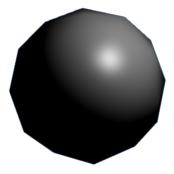
\includegraphics[width=.3\linewidth]{figures/smooth.png}
		\label{fig:demo-fancy}}
	\caption{\label{fig:demo} 
		Caption}
\end{figure}

\subsection{Equations}
\begin{equation}
	\mathcal{L} = \frac{1}{n}\sum_n^{i=1} (Y_i - \hat{Y}_i)^2
\end{equation}

\subsection{Comments/Labels}
% TODO - this is a todo

% APPENDIX
\appendix
\section{Python Code}
This would be our appendix.

% end document
\end{document}
